% Build with XeLaTeX from TestSkill2/docs. No original-project assets are copied.
\documentclass[11pt,a4paper]{article}
\usepackage[margin=20mm,headheight=15pt]{geometry}
\usepackage{fontspec}
\setmainfont{Arial}
\setsansfont{Arial}
\setmonofont{Consolas}[Scale=0.84]
\usepackage{graphicx,xcolor,booktabs,tabularx,array,enumitem,fancyhdr,titlesec,hyperref}
\definecolor{Ink}{HTML}{292524}
\definecolor{Coral}{HTML}{C35D49}
\definecolor{Muted}{HTML}{625B55}
\definecolor{Cream}{HTML}{F7E9D7}
\hypersetup{colorlinks=true,linkcolor=Coral,urlcolor=Coral,pdftitle={GiaoNong — Tăng số đơn và chất lượng giao hàng},pdfauthor={Supervisor dự án}}
\urlstyle{tt}
\color{Ink}
\setlength{\parindent}{0pt}
\setlength{\parskip}{6pt}
\renewcommand{\arraystretch}{1.25}
\setlist[itemize]{leftmargin=*,nosep,topsep=4pt}
\pagestyle{fancy}
\fancyhf{}
\fancyhead[L]{\small\textcolor{Muted}{GIAONONG / PHÂN TÍCH KINH DOANH}}
\fancyhead[R]{\small\textcolor{Muted}{08/10/2026}}
\fancyfoot[L]{\footnotesize\textcolor{Muted}{Phân tích đơn hàng · 01/03–31/08/2026}}
\fancyfoot[R]{\small\thepage}
\renewcommand{\headrulewidth}{0.3pt}
\titleformat{\section}{\Large\bfseries\color{Coral}}{\thesection}{0.6em}{}
\titleformat{\subsection}{\normalsize\bfseries}{\thesubsection}{0.6em}{}
\newcolumntype{Y}{>{\raggedright\arraybackslash}X}
\newcommand{\file}[1]{\nolinkurl{#1}}
\newcommand{\shot}[2]{\includegraphics[width=\linewidth]{#1}\par{\small\textcolor{Muted}{#2}}\par\medskip}
\begin{document}
\thispagestyle{empty}
{\small\bfseries\textcolor{Coral}{BÁO CÁO KINH DOANH · GIAONONG · 08/10/2026}}\par
\vspace{4mm}
{\LARGE\bfseries Số đơn tăng, nhưng hủy và trễ\\đang làm giảm chất lượng tăng trưởng\par}
\vspace{3mm}
{\large Kỳ 01/03–31/08/2026 · Đề xuất ưu tiên rà ca Tối\par}
\vspace{4mm}

\textbf{Thông điệp cho cuộc họp.} Tháng 8 ghi nhận 1.144 đơn, cao hơn tháng 3 khoảng 24,35\%. Trong cùng phép so, tỷ lệ trễ tăng từ 5,97\% lên 25,08\%, tỷ lệ hủy từ 3,48\% lên 12,85\%. Số đơn ghi nhận tăng không đồng nghĩa trải nghiệm giao hàng được cải thiện. Cần nhìn phần vận hành cùng tổng đơn.

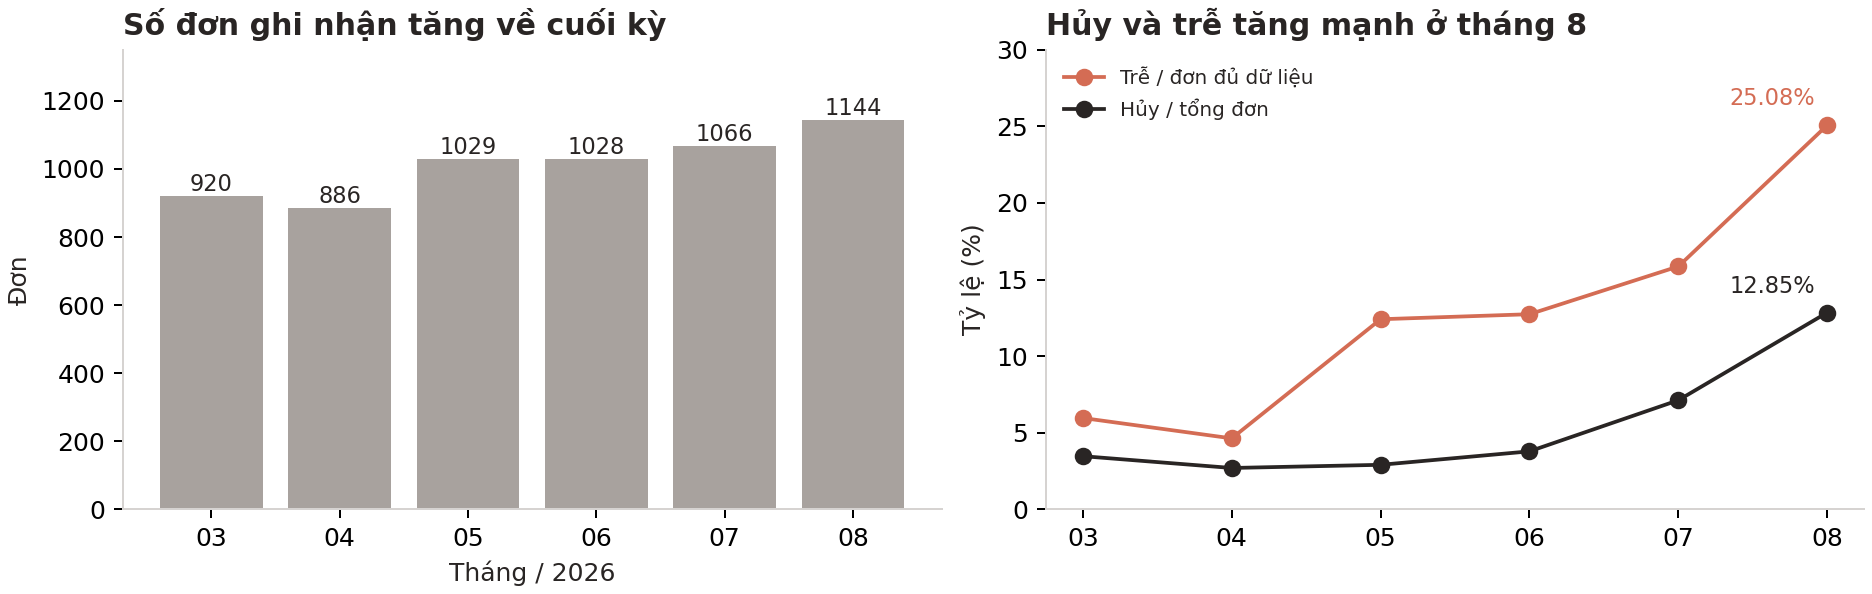
\includegraphics[width=\linewidth]{../reports/business_report/monthly_story.png}

{\small\textcolor{Muted}{Hình 1. Trễ chia cho đơn hoàn thành đủ dữ liệu; hủy chia cho tổng đơn. So tháng 3 với tháng 8 chưa loại ảnh hưởng mùa vụ hoặc cơ cấu đơn.}}

\begin{tabularx}{\linewidth}{YYY}
\toprule
\textbf{24,35\%} & \textbf{19,11 điểm \%} & \textbf{52,13\%}\\
Mức tăng đơn tháng 8 so tháng 3 & Mức tăng tỷ lệ trễ giữa hai tháng & Phần đơn trễ toàn kỳ thuộc ca Tối\\
\bottomrule
\end{tabularx}

\textbf{Vấn đề kinh doanh.} Đơn hủy không có thu nhập ghi nhận nhưng vẫn có bồi thường. Giao trễ đi cùng điểm đánh giá thấp hơn. Vì vậy, tổng đơn chưa đủ để đánh giá kết quả: cần xem đồng thời lượng đơn, chất lượng giao, tiền ghi nhận và trải nghiệm khách. Chưa có dữ liệu để quy đổi thành tiền mất đi trong tương lai.

\textbf{Đề xuất cần chốt.} Cho phép rà ca Tối và thử một thay đổi trong phạm vi nhỏ, đo trước–sau với nhóm so sánh phù hợp. Chưa có căn cứ tăng người đồng loạt, giảm phạm vi giao hoặc hứa mức tiết kiệm.

\newpage
\section{Ưu tiên ca Tối vì quy mô vấn đề}
Toàn kỳ có 750 đơn trễ trên 5.725 đơn đủ dữ liệu. Ca Tối có 391 đơn trễ, chiếm 52,13\% số trễ, và 198/348 đơn hủy, chiếm 56,90\% số hủy. Tỷ lệ trễ ca này là 20,19\% trên 1.937 đơn đủ dữ liệu. Đây là điểm bắt đầu có quy mô lớn và đầu mối vận hành rõ, không chỉ là nhóm có tỷ lệ cao.

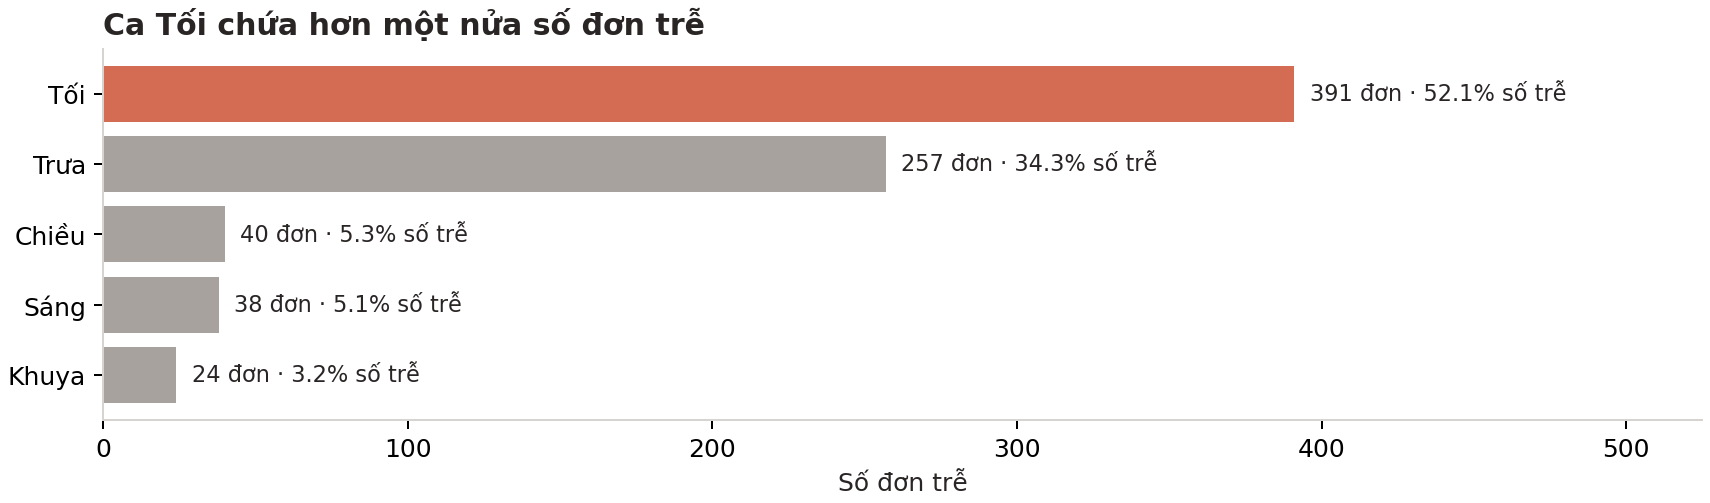
\includegraphics[width=\linewidth]{../reports/business_report/evening_priority.png}
{\small\textcolor{Muted}{Hình 2. Đóng góp vào 750 đơn trễ toàn kỳ. Khung giờ phân hoạch đơn nên cộng được; không cộng các nhóm mưa/khoảng cách vào đây.}}

\subsection{Chia theo mưa để nhìn rõ hơn cơ cấu}
\begin{tabularx}{\linewidth}{Yrrr}
\toprule
\textbf{Nhóm quan sát} & \textbf{Đủ dữ liệu} & \textbf{Trễ} & \textbf{Tỷ lệ trễ}\\
\midrule
Khung khác, không mưa & 2.446 & 114 & 4,66\%\\
Tối, không mưa & 1.278 & 167 & 13,07\%\\
Khung khác, mưa & 1.342 & 245 & 18,26\%\\
Tối, mưa & 659 & 224 & 33,99\%\\
\bottomrule
\end{tabularx}
Ca Tối có tỷ lệ trễ cao hơn các khung khác trong cả nhóm mưa và không mưa. Điều này giúp chọn nơi tìm hiểu, chưa chứng minh ca Tối hoặc mưa gây trễ: khoảng cách, khu vực, nhà hàng và tháng có thể khác nhau giữa nhóm.

\subsection{Đơn xa cần rà tiếp, chưa đủ để đổi chính sách giao}
Nhóm từ 6 km có 250/439 đơn trễ, tương đương 56,95\%; dưới 2 km là 53/1.232, tương đương 4,30\%. Nhóm xa có tỷ lệ đáng chú ý nhưng số trễ thấp hơn ca Tối. Nên xem các đơn xa tập trung ở ca/khu vực nào trước khi đổi chính sách. Tối, mưa và xa có thể chồng nhau; không cộng 391+469+250 thành số đơn có vấn đề.

\newpage
\section*{Dashboard: nhìn toàn cảnh rồi khoanh điểm nghẽn}
\shot{../reports/phase5c/final_reopen/Tổng quan.png}{\textbf{Tổng quan — tăng trưởng có đi cùng chất lượng?} Trang này đặt lượng đơn cạnh hủy và trễ theo tháng, khung giờ và khu vực. Dùng để xác định nơi cần hỏi sâu; kết hợp tỷ lệ với số đơn để tránh ưu tiên một nhóm quá nhỏ.}
\shot{../reports/phase5c/final_reopen/Vận hành.png}{\textbf{Vận hành — nên rà ca và điều kiện giao nào trước?} Ca Tối, mưa và nhóm từ 6 km đều có tỷ lệ trễ đáng chú ý. Trang này hỗ trợ khoanh phạm vi rà quy trình; các nhóm có thể chồng nhau và chưa chứng minh nguyên nhân.}
{\footnotesize\textcolor{Muted}{Ảnh chụp dashboard Power BI của Pilot 2 sau mở lại. Kỳ phân tích là tháng 3–8/2026; không diễn giải các điểm 0 ngoài kỳ trên trục tháng là hoạt động kinh doanh thực tế.}}

\newpage
\section{Hủy và trễ liên quan tới tiền và trải nghiệm}
\subsection{Đơn hủy ít, nhưng tập trung phần lớn bồi thường}
348 đơn hủy chiếm 5,73\% tổng đơn nhưng mang 7,224 triệu bồi thường, tương đương 72,25\% tổng bồi thường 9,999 triệu theo đơn vị nguồn. Thu nhập ghi nhận của nhóm hủy bằng 0. Đây là khoản đã quan sát, đáng rà quy trình hủy; chưa phải toàn bộ chi phí hoặc doanh thu mất đi do hủy.

198/348 đơn hủy mang lý do “Chờ tài xế quá lâu”, tương đương 56,90\%. Nhãn nguồn này gợi hướng kiểm thời điểm chờ/phân công. Chưa xác minh độc lập và không suy 198 đơn ấy chính là toàn bộ 198 đơn hủy ca Tối.

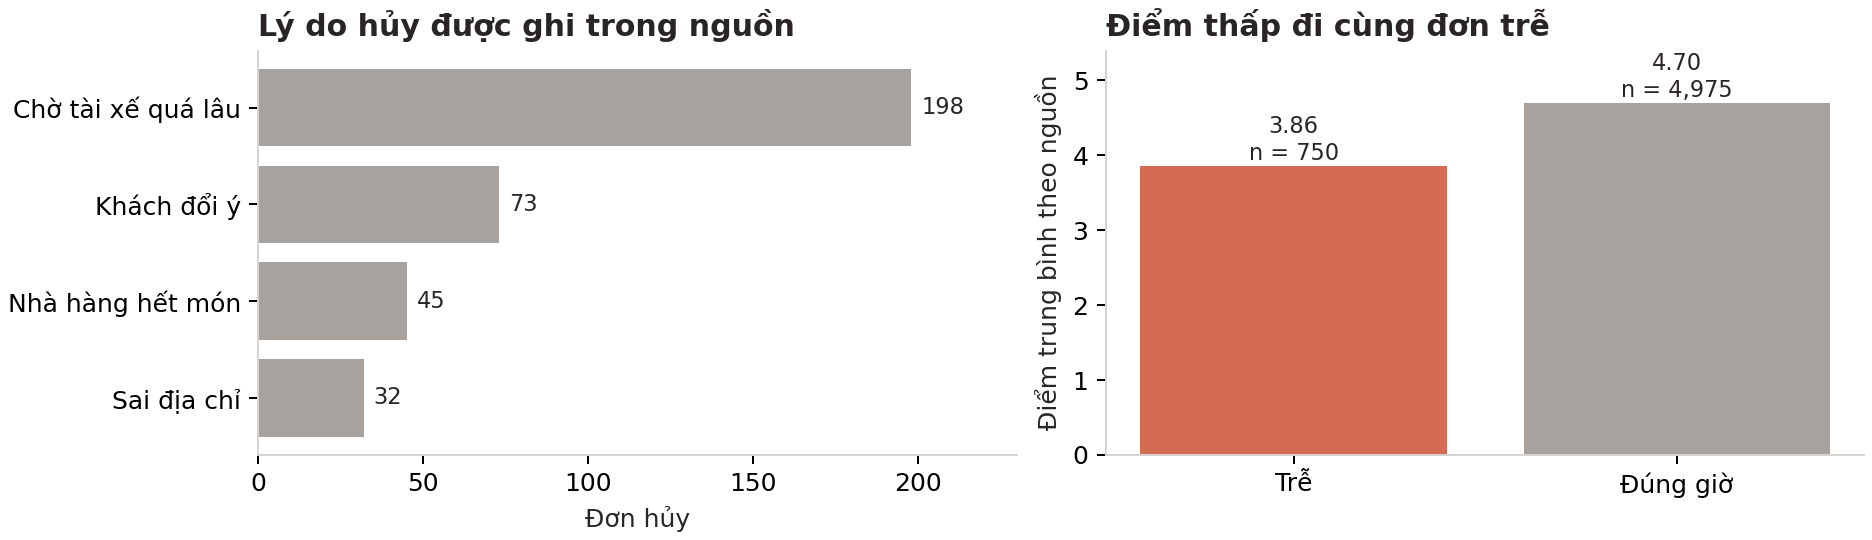
\includegraphics[width=\linewidth]{../reports/business_report/business_impact.png}
{\small\textcolor{Muted}{Hình 3. Lý do hủy và điểm đơn hoàn thành. Hai biểu đồ mô tả nhóm riêng, chưa xác định nguyên nhân.}}

\subsection{Điểm thấp đi cùng trễ; chưa đo khách rời bỏ}
Điểm trung bình của 750 đơn trễ là 3,86, so với 4,70 ở 4.975 đơn đúng giờ: chênh 0,84 điểm. Chất lượng giao đáng được theo dõi cùng phản hồi khách. Chưa có thiết kế kiểm nguyên nhân hoặc lịch sử sau kỳ để kết luận trễ làm khách ngừng mua.

Có 1.261/2.098 khách đặt từ hai đơn trong kỳ, tương đương 60,10\%. Đây là mua lặp lại trong sáu tháng, chưa là giữ chân. Muốn đo ảnh hưởng lâu dài cần theo dõi khách sau lần trễ và so nhóm tương đồng.

\subsection{Cải thiện chất lượng cần đi cùng kiểm chi phí}
Toàn kỳ ghi nhận 203,34 triệu thu nhập và 50,86 triệu chênh lệch;1.320/6.073 đơn có chênh lệch âm. Tăng nguồn lực để giảm trễ có thể tăng chi phí. Thử nghiệm cần theo dõi bồi thường/đơn và chi phí phát sinh cùng chất lượng. Đơn vị tiền và phạm vi chi phí chưa được xác nhận để gọi là lợi nhuận kế toán.

\newpage
\section*{Dashboard: kiểm đánh đổi về tiền và khách hàng}
\shot{../reports/phase5c/final_reopen/Tài chính.png}{\textbf{Tài chính — cải thiện giao hàng có kiểm soát chi phí không?} Trang này đặt thu nhập, chênh lệch ghi nhận và đơn âm cạnh nhau, theo tháng/khu vực. 1.320 đơn âm là tín hiệu cần rà trước khi tăng chi phí; chưa đủ để kết luận lãi kế toán hoặc tiền có thể tiết kiệm.}
\shot{../reports/phase5c/final_reopen/Khách hàng.png}{\textbf{Khách hàng — chất lượng giao đi cùng trải nghiệm thế nào?} Điểm nhóm trễ thấp hơn nhóm đúng giờ, còn 60,10\% khách có từ hai đơn trong kỳ. Dùng để theo dõi trải nghiệm cùng vận hành; mua lặp lại trong kỳ chưa chứng minh giữ chân khách lâu dài.}
{\footnotesize\textcolor{Muted}{Bốn trang dashboard là công cụ xem và khoanh vấn đề. Các biểu đồ phân tích và bảng số trong báo cáo bổ sung mức chi tiết cần cho đề xuất quản lý.}}

\newpage
\section{Thử nghiệm ca Tối và quyết định đề nghị quản lý}
\subsection{Kiểm một cách cải thiện trước khi triển khai rộng}
Đề xuất rà đơn ca Tối rồi chọn \textbf{một} thay đổi, chẳng hạn điều chỉnh thời điểm/phương thức phân công tài xế trong phạm vi nhỏ. Cách làm phải dựa trên kết quả rà thời gian chờ và quy trình thực tế. Nếu nguyên nhân khác, chọn xử lý tương ứng; chưa có căn cứ khẳng định thiếu tài xế.

{\small
\begin{tabularx}{\linewidth}{p{22mm}YY}
\toprule
\textbf{Lịch đề xuất} & \textbf{Việc làm} & \textbf{Đầu mối / đầu ra}\\
\midrule
Tuần 1 & Chốt ranh giờ, định nghĩa trễ, dữ liệu phân công, đơn vị tiền; chọn vùng thử và kỳ so sánh & Vận hành cùng chủ dữ liệu chốt phạm vi và mức hiện tại\\
Tuần 2–3 & Thử một thay đổi, ghi lượng đơn, mưa, khoảng cách và chi phí theo cùng cách đo & Vận hành thực hiện; DA theo dõi nhóm thử/so sánh\\
Tuần 4 & So kết quả cùng phạm vi và điều kiện tương đồng; rà đánh đổi/độ ổn định & DA báo cáo; quản lý quyết định tiếp tục, điều chỉnh hoặc dừng\\
\bottomrule
\end{tabularx}}

Đây là lịch đề xuất để thảo luận, chưa được duyệt. Nếu ít đơn hoặc nhóm không tương đồng, kéo dài quan sát hoặc kết luận chưa đủ bằng chứng; không chọn phép so để đạt kết quả mong muốn.

\subsection{Cách đo trước–sau}
\begin{itemize}
\item \textbf{Chất lượng:} trễ/đơn đủ dữ liệu, hủy/tổng đơn trong cùng ca/vùng; báo cả tử số và mẫu số.
\item \textbf{Đánh đổi:} bồi thường/đơn, chi phí thêm và lượng đơn xử lý; tỷ lệ đẹp hơn chưa đủ nếu mẫu ít hoặc chi phí tăng quá lớn.
\item \textbf{Trải nghiệm:} điểm kèm số đánh giá và phản hồi; mua lặp lại chỉ đánh giá khi có kỳ theo dõi phù hợp.
\end{itemize}
20,19\% trễ ca Tối của sáu tháng chỉ giúp chọn ưu tiên. Mức trước thử phải tính lại trên đúng vùng/kỳ/điều kiện; xem cơ cấu mưa, khoảng cách và loại đơn của nhóm so sánh. Chưa đặt target phần trăm hoặc ROI.

\subsection{Ba quyết định cần chốt}
\textbf{1.} Chọn người phụ trách ca Tối và cho phép rà quy trình/dữ liệu phân công.\\
\textbf{2.} Chốt vùng thử, một thay đổi và mức chi phí chấp nhận được.\\
\textbf{3.} Thống nhất cách đo, điều kiện đủ dữ liệu và thời điểm review trước mở rộng.

\newpage
\section{Phương pháp và giới hạn của kết luận}
\subsection{Từ câu hỏi quản lý tới bằng chứng}
Câu hỏi chính: \textbf{nhóm nào cần rà trước để cải thiện giao hàng mà vẫn kiểm soát chi phí?} Nguồn có 6.073 đơn duy nhất trong 184 ngày liên tục,2.098 khách và 8 khu vực. Phân tích tháng tìm biến động; khung giờ tìm nơi tập trung vấn đề; chia ca Tối theo mưa kiểm một phần khác biệt cơ cấu.

Tỷ lệ dùng nhóm đủ dữ liệu; đóng góp dùng số đơn để không chọn một nhóm nhỏ chỉ vì tỷ lệ cao. Nhóm khung giờ–mưa giúp nhìn cụ thể hơn nhưng chưa thay kiểm khoảng cách, vùng hoặc tháng. Chuẩn hóa nhóm khoảng cách để đơn đúng 6 km thuộc nhóm từ 6 km trở lên.

\subsection{Kỹ thuật giúp phép đo đúng câu hỏi}
Python đọc CSV, tính tổng hợp độc lập và tạo ba biểu đồ. Chuẩn hóa giữ giá trị gốc, đơn hủy, ô thiếu và chênh lệch âm. Power Query/M nạp bảng; model Power BI nối đơn với ngày, khách và các nhóm; DAX tính chỉ số theo lựa chọn. Công cụ hỗ trợ phép đo, còn ưu tiên dựa trên quy mô vấn đề, ảnh hưởng và khả năng thử.

Xem cả trung bình và trung vị để một số đơn rất lâu không làm lệch nhận xét. Chờ tài xế trung bình 6,17 phút, trung vị 4,60 phút trên 5.725 đơn hoàn thành: có nhóm chờ lâu đáng rà. Chưa xác nhận các bước chồng nhau nên không cộng chúng thành công thức mới hoặc kết luận bên nào gây trễ.

\subsection{Giới hạn ảnh hưởng quyết định}
\begin{itemize}
\item \textbf{Nhân quả:} chênh lệch là quan sát; chưa kiểm độc lập tác động của ca Tối, mưa, khoảng cách và cơ cấu đơn.
\item \textbf{Chuẩn vận hành:} chưa đủ định nghĩa trễ/mưa/khung giờ để tự đặt thời gian cam kết hoặc kết luận vi phạm.
\item \textbf{Tiền:} dùng đơn vị nguồn và chi phí được ghi; chưa là lãi kế toán hoặc tiền có thể tiết kiệm.
\item \textbf{Khách/thời gian:} chỉ có tháng 3–8/2026; chưa suy giữ chân/rời bỏ hoặc xu hướng dài hạn, chưa loại mùa vụ khi so hai tháng.
\end{itemize}

\textbf{Phân tích đã chỉ ra:} ca Tối là điểm bắt đầu có quy mô lớn; bồi thường tập trung ở hủy; điểm thấp đi cùng trễ. \textbf{Kết quả vận hành cần đo tiếp:} thử nghiệm chưa diễn ra, nên chưa có mức giảm trễ, tiết kiệm hoặc giữ chân khách được chứng minh.

\newpage
\section{Phụ lục số liệu cho cuộc họp}
\subsection{Biến động theo tháng}
{\small
\begin{tabularx}{\linewidth}{Yrrrrr}
\toprule
\textbf{Tháng} & \textbf{Đơn} & \textbf{Hủy} & \textbf{Tỷ lệ hủy} & \textbf{Trễ / đủ dữ liệu} & \textbf{Tỷ lệ trễ}\\
\midrule
03/2026 & 920 & 32 & 3,48\% & 53 / 888 & 5,97\%\\
04/2026 & 886 & 24 & 2,71\% & 40 / 862 & 4,64\%\\
05/2026 & 1.029 & 30 & 2,92\% & 124 / 999 & 12,41\%\\
06/2026 & 1.028 & 39 & 3,79\% & 126 / 989 & 12,74\%\\
07/2026 & 1.066 & 76 & 7,13\% & 157 / 990 & 15,86\%\\
08/2026 & 1.144 & 147 & 12,85\% & 250 / 997 & 25,08\%\\
\bottomrule
\end{tabularx}}

\subsection{Số nền và cách tính}
{\small
\begin{tabularx}{\linewidth}{p{41mm}p{31mm}Y}
\toprule
\textbf{Chỉ số} & \textbf{Toàn kỳ} & \textbf{Phạm vi / mẫu số}\\
\midrule
Tổng đơn & 6.073 & Một dòng = một đơn duy nhất\\
Hủy & 348 / 5,73\% & Cờ hủy 1 / tổng đơn\\
Trễ & 750 / 13,10\% & Cờ trễ 1 /5.725 đơn đủ dữ liệu\\
Thu nhập ghi nhận & 203.341.200 & Tổng revenue, đơn vị nguồn\\
Chênh lệch ghi nhận & 50.859.200 & Tổng profit, chưa là lãi kế toán đầy đủ\\
Chênh lệch âm & 1.320 / 21,74\% & Đơn profit âm / tổng đơn\\
Bồi thường đơn hủy & 7.224.000 & Tổng compensation của 348 đơn hủy\\
Tổng bồi thường & 9.999.000 & Tổng compensation của 6.073 đơn\\
Khách từ hai đơn & 1.261 / 60,10\% & Trong 2.098 khách của kỳ; không cộng nhóm khách\\
Điểm trung bình & 4,59 & 5.725 đơn hoàn thành có điểm\\
\bottomrule
\end{tabularx}}

\subsection{Nguồn số liệu}
CSV người dùng cung cấp trong TestSkill 2 là đầu vào. Số báo cáo tính trực tiếp từ \file{data/curated/orders.csv}; tháng, khung giờ, mưa và khoảng cách đối chiếu với bảng phân tích đã lưu. Khung giờ–mưa và đóng góp bồi thường được tính thêm để trả lời câu hỏi quản lý.

Chi tiết: \file{reports/business_report/summary.json}; phép tính/biểu đồ: \file{scripts/business_report.py}; định nghĩa chỉ số: \file{reports/phase4/registry.json}. Hướng dẫn sử dụng và hồ sơ kỹ thuật lưu riêng.
\end{document}
